\documentclass[xetex,mathserif,serif]{beamer}

% Hyperlinks.
\usepackage{hyperref}

% Language settings.
\usepackage{polyglossia}
\setdefaultlanguage[babelshorthands=true]{russian}

% Setting outer theme.
\useoutertheme{infolines}

% Setting font.
\usepackage{fontspec}
\setmainfont{FreeSans}
\newfontfamily{\russianfonttt}{FreeSans}

% Code highlighting.
\usepackage[outputdir=temp]{minted}
\usepackage{xcolor}

% Images.
\usepackage{graphicx}
\usepackage{animate}
\usepackage{subfig}


\usepackage{mathtools}

\title{Поиск похожих изображений}
\author[Александр Смирнов]{Александр Смирнов}
\date{22.09.2020}

\begin{document}


\begin{frame}
	\titlepage{}
\end{frame}


\begin{frame}
	\frametitle{Задача}

	\begin{itemize}
		\item Поиск по изображениям
		\item Каждому изображению сопоставить набор тегов и искать по тегам
		      \begin{itemize}
			      \item не масштабируется на новые изображения
		      \end{itemize}
		\item Предоставить пример изображения и запросить похожие
	\end{itemize}

	\begin{figure}[b]
		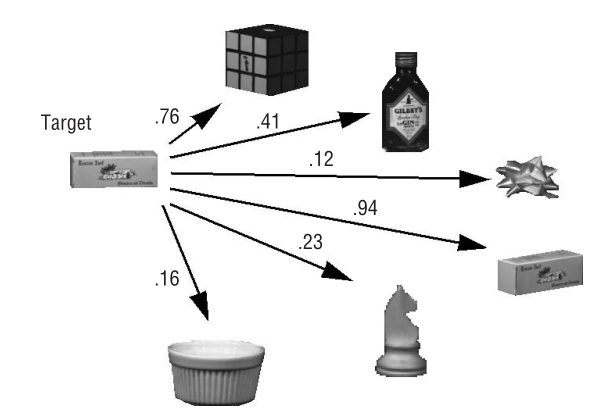
\includegraphics[width=0.4\textwidth]{./images/query_sample.png}
		\centering
	\end{figure}
\end{frame}


\begin{frame}
	\frametitle{Решение}

	\begin{itemize}
		\item Выделим признаки из нашего изображения и сравним с признаками остальных изображений
		\item Можно заранее выделить признаки из базы изображений
	\end{itemize}
\end{frame}


\begin{frame}
	\frametitle{Цветовые признаки}

	\begin{itemize}
		\item Самая простая модель -- уменьшить количество цветов на изображении и считать, насколько часто появляется каждый цвет
		      \begin{itemize}
			      \item часто используется для исключение кандидатов из рассмотрения
		      \end{itemize}
		\item Среднее значение по цветам
	\end{itemize}
\end{frame}


\begin{frame}
	\frametitle{Дерево квадрантов}

	\begin{itemize}
		\item У каждого корня 4 потомка
		\item Проходимся по изображению, берем каждые 4 пикселя и сжимаем их в один, с цветом равным среднему
		\item Сравниваем по векторам цветов
		      \begin{itemize}
			      \item корневой узел содержит в себе среднее значение по цветам
			      \item 1 слой содержит в себе 4 пикселя, это вектор из 12 элементов
			      \item 2 слой -- 16 пикселей: 48 элементов
		      \end{itemize}
	\end{itemize}
\end{frame}


\begin{frame}
	\frametitle{Дерево квадрантов}

	\begin{figure}[]
		\centering
		\subfloat{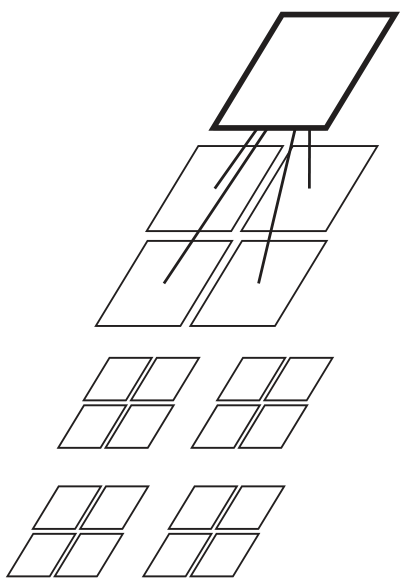
\includegraphics[width=0.3\textwidth]{./images/quadtree_graph.png}}
		\hfill
		\subfloat{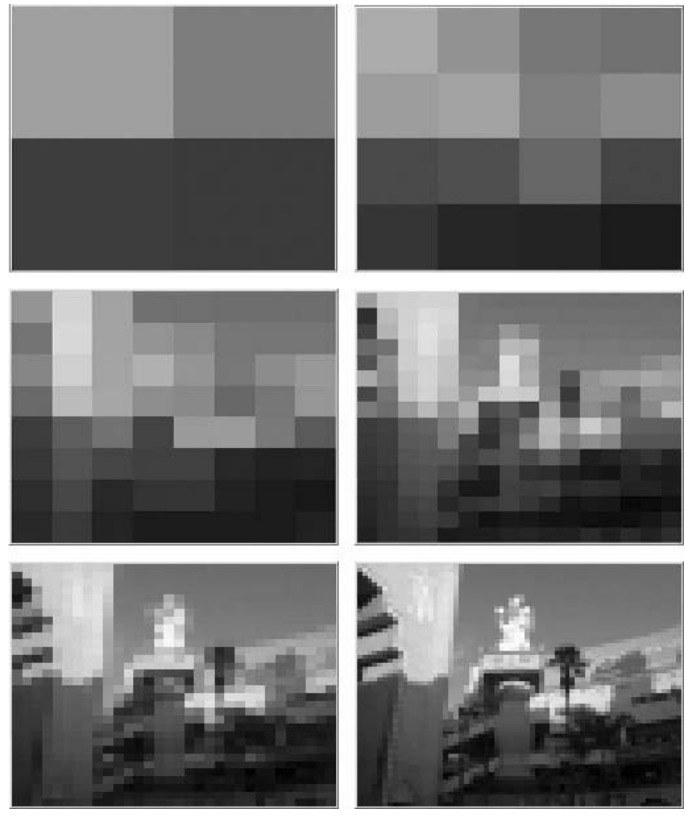
\includegraphics[width=0.4\textwidth]{./images/quadtree_picture.png}}
	\end{figure}
\end{frame}


\begin{frame}
	\frametitle{Гистограммы тона и насыщенности}

	\begin{itemize}
		\item Тон -- направление вектора на диаграмме цветности с началом в точке белого и концом в данной цветности
		      \begin{itemize}
			      \item \begin{figure}[h]
				            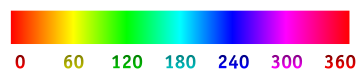
\includegraphics[width=0.5\textwidth]{./images/hue.png}
				            \centering
			            \end{figure}
		      \end{itemize}
		\item Насыщенность -- насколько цвет отличен от серого
	\end{itemize}
\end{frame}


\begin{frame}
	\frametitle{Гистограммы тона и насыщенности}

	\begin{figure}[h]
		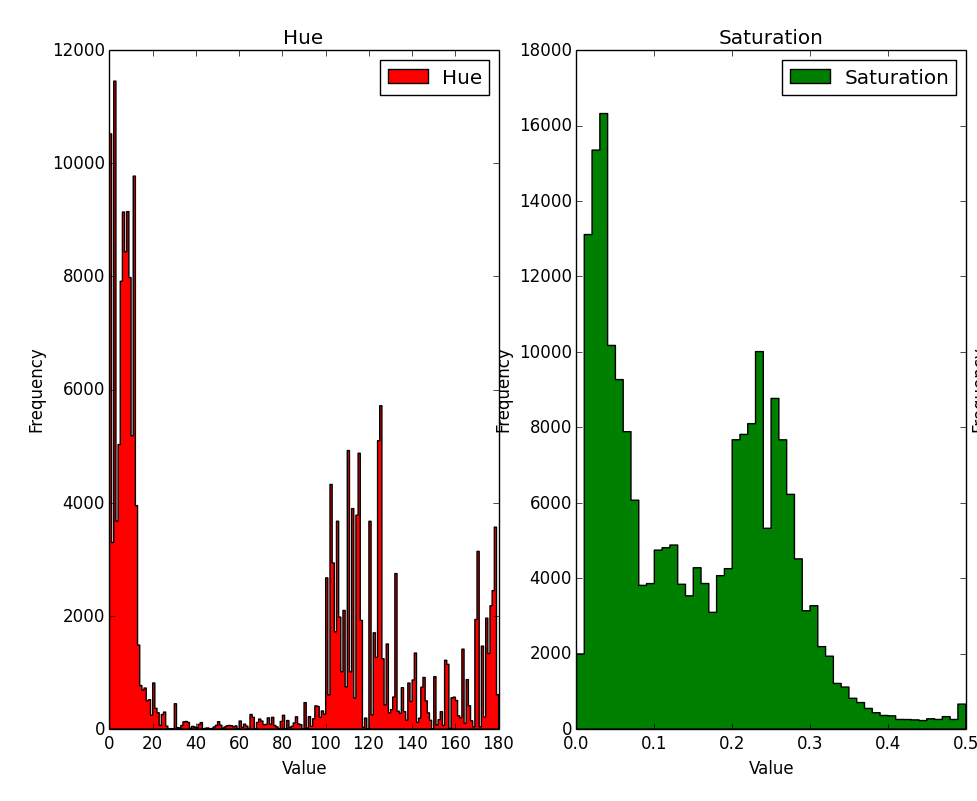
\includegraphics[width=0.7\textwidth]{./images/hue_saturation.png}
		\centering
	\end{figure}
\end{frame}


\begin{frame}
	\frametitle{Распознавание границ}

	\begin{itemize}
		\item Находим границы по разнице в интенсивности рядом стоящих пикселей
		      \begin{itemize}
			      \item проходимся матрицами свёртки по каждому пикселю изображения, изменяя его интенсивность
			      \item
			            $$s_{x}=\begin{matrix}
					            -1 & 0 & 1 \\
					            -2 & 0 & 2 \\
					            -1 & 0 & 1
				            \end{matrix}$$

			            $$s_{y}=\begin{matrix}

					            -1           & -2           & -1           \\
					            \phantom{-}0 & \phantom{-}0 & \phantom{-}0 \\
					            \phantom{-}1 & \phantom{-}2 & \phantom{-}1
				            \end{matrix}$$
		      \end{itemize}
		\item Сравниваем вектора границ
	\end{itemize}
\end{frame}


\begin{frame}
	\frametitle{Распознавание границ}

	\begin{figure}[]
		\centering
		\subfloat{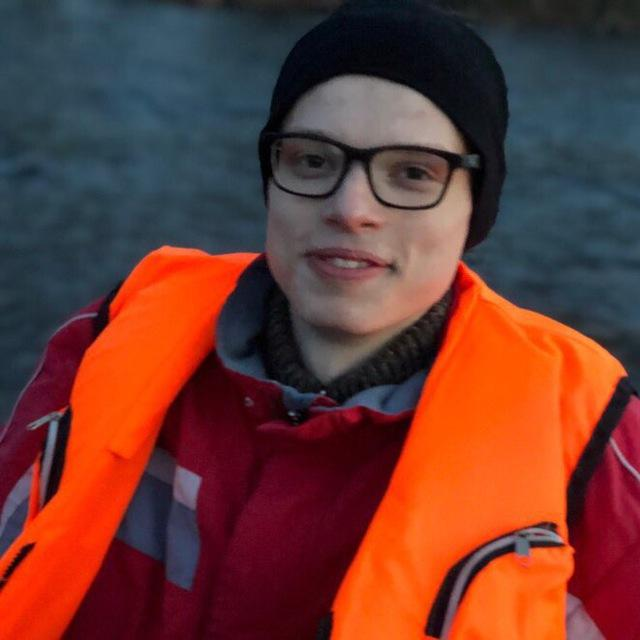
\includegraphics[width=0.4\textwidth]{./images/me.jpg}}
		\hfill
		\subfloat{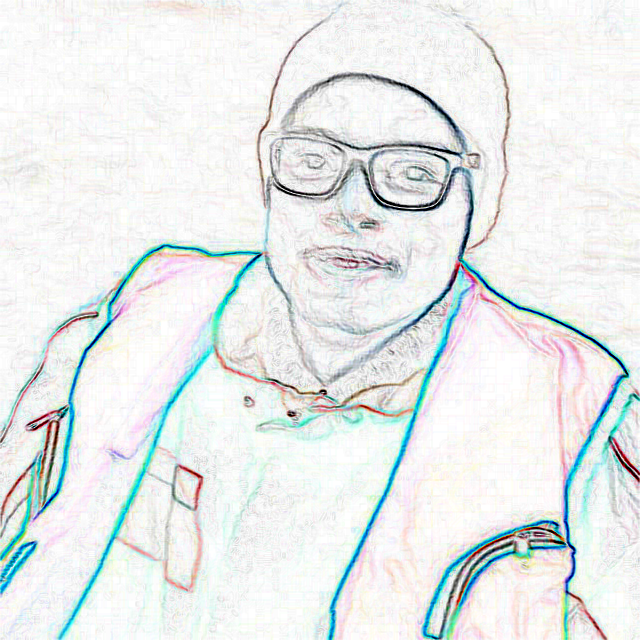
\includegraphics[width=0.4\textwidth]{./images/me_edged.png}}
	\end{figure}
\end{frame}


\begin{frame}
	\frametitle{Дробление на части}

	\begin{itemize}
		\item Высчитываем признаки отдельно для каждой части и сливаем их в единое множество признаков
		\item Увеличиваем приоритет пикселей в центре изображения
	\end{itemize}
\end{frame}


\begin{frame}
	\frametitle{Дробление на части}

	\begin{figure}[h]
		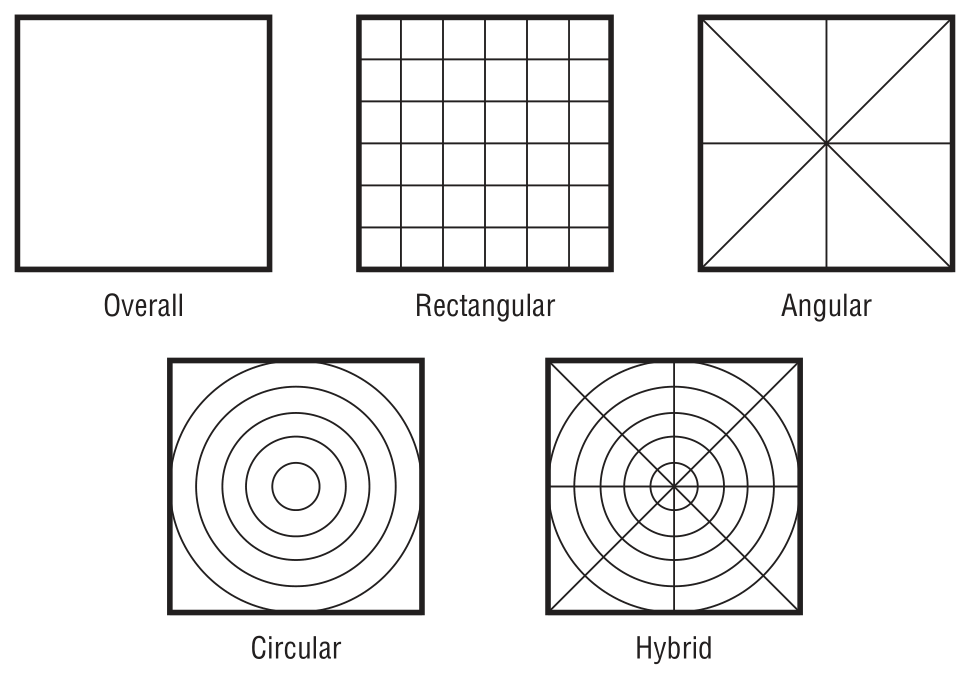
\includegraphics[width=0.7\textwidth]{./images/spartial.png}
		\centering
	\end{figure}
\end{frame}


\begin{frame}
	\frametitle{Однородноть}

	\begin{itemize}
		\item Изменения в интенсивности цвета
	\end{itemize}


	\begin{figure}[h]
		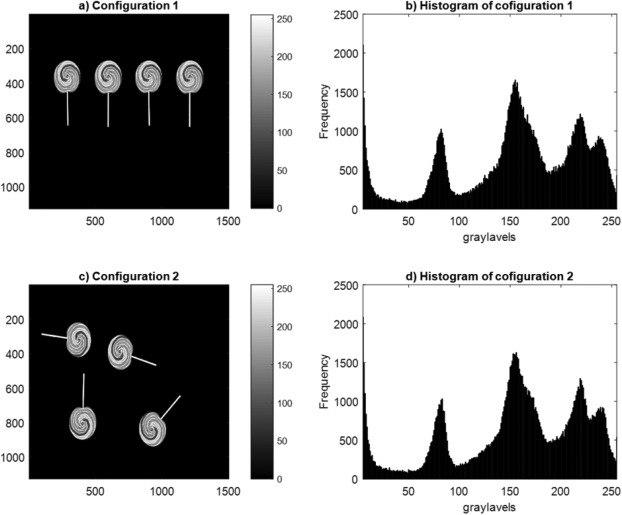
\includegraphics[width=0.5\textwidth]{./images/heter.jpg}
		\centering
	\end{figure}
\end{frame}


\begin{frame}
	\frametitle{Сегментация}

	\begin{itemize}
		\item Разделение на сегменты
		\item Выделение фона
	\end{itemize}


	\begin{figure}[h]
		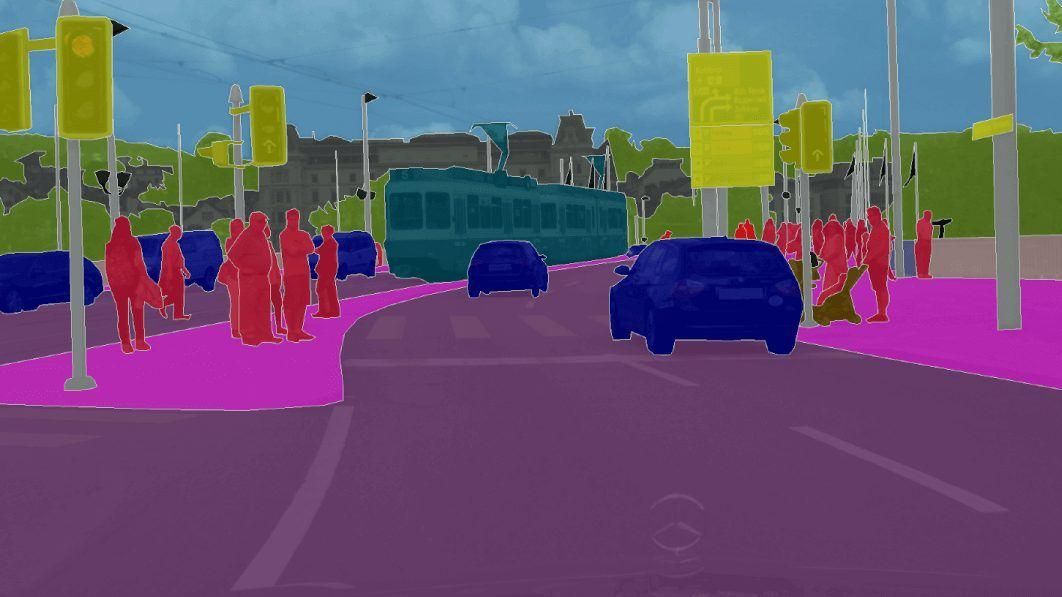
\includegraphics[width=0.5\textwidth]{./images/segm.jpg}
		\centering
	\end{figure}
\end{frame}


\begin{frame}
	\frametitle{Глубокое обучение}

	\begin{itemize}
		\item Свёрточная нейронная сеть для выделения признаков
		      \begin{itemize}
			      \item принимает вектор изображения, возвращает вектор признаков
			      \item путем демонстрации алгоритму множества размеченных данных мы хотим подобрать коэффиценты так, чтобы вектора признаков похожих изображений находились рядом в пространстве признаков
		      \end{itemize}
		\item Сравниваем расстояние между вектором признаков искомого изображения и остальных изображений
	\end{itemize}
\end{frame}


\end{document}
